\chapter{More group structure of the cube}\label{chap:structure}
In this chapter, we dive into more details about the group structure of Rubik's Cubes and explain how to find the group size of an arbitrarily large Rubik's Cube. While giving the definition of the semi-direct group, we illustrate the explicit structure of $G_3$ to build up for the next chapter.

\section{Size of the Rubik's Cube group}
\par In Chapter~\ref{chap:encryption}, we mentioned that there exist some illegal states of the Rubik's Cube $C_3$ and thus the group $G_3$ constructed by states of $C_3$ is a subgroup of $S_{48}$. We now want to show how to find the size of group $G_3$ and we expand the method to illustrate how to calculate size of group $G_n$ constructed by an arbitrary large cube $C_n$.
\par Recall Figure~\ref{fig:cube-type}, we showed that there are 8 corner cubes in $C_3$. The 8 corner cubes can freely exchange their locations and they can be arranged in $8!$ ways. When we fix locations of the 8 corner cubes, each of them can be arranged in 3 different orientations, giving $3^8$ possibilities for each ordering of the corner pieces. Similarly, there are 12 edge cubes that can freely exchange their locations and the can be arranged in $12!$ ways. When we fix locations of the 12 edge cubes, each of them can be arranged in 2 different orientations, giving $2^{12}$ possibilities for each permutation of the edge cubes. However, further reductions are required due to the structure of the Rubik's Cube.
\par The reason we need to further reduce the group size is explicitly explained in Chapter 11 in paper\cite{janet}. We will not repeat all the details presented there but give the essential part of the argument. For the 8 corner cubes of $C_3$, only 7 of them can be oriented independently, meaning the orientation of the 8th corner cube depends on the preceding seven. Hence, when we fix locations for all 8 corner cubes, they can have at most $3^7$ possible different orientations. Similarly, when we determine orientations for 11 of the 12 edge cubes, the orientation of the last edge cube will be fixed. It follows that there are $2^{11}$ possible orientations for each permutation of the edge cubes. So for now, the order of $C_3$ can be calculated as $8! \cdot 3^7 \cdot 12! \cdot 2^{11}$. In \cite{janet}, a labelling system on the cube was created, and the authors proved that any permutation of the edges must be an even permutation. Therefore we must reduce this number by half. Finally, we find the order of $C_3$ is $8! \cdot 3^7 \cdot 12! \cdot 2^{10} = 43,250,003,274,489,856,000$.
\par For a hint of the proof for above statements, recall that in Chapter~\ref{chap:encryption}, we defined each valid state as a shuffling result of a series of fundamental moves. By analyzing properties of those permutations, we can obtain a good understanding on how to determine if a state of $C_3$ is valid.
\par Now we can explain how to find group order of $G_n$ for a arbitrarily large cube $C_n$. The calculation for corner cubes will stay true for any cube $C_n$ but the calculation for edge cubes will change since cubes with different side lengths have different number of edge cubes and for larger cubes, there will be two types of edge cubes. We also need to introduce a couple more different small cubes with single visible colored piece. We can use $C_7$ to illustrate all types of small cubes. Consider Figure~\ref{fig:7-center-corner} as one face of the cube. The small cubes colored in blue are the corner cubes and those colored in yellow are the fixed center cubes. Those small cubes behave the same as they are in $C_3$.
\begin{figure}[ht]
    \centering
    \begin{minipage}{0.45\textwidth}
        \centering
        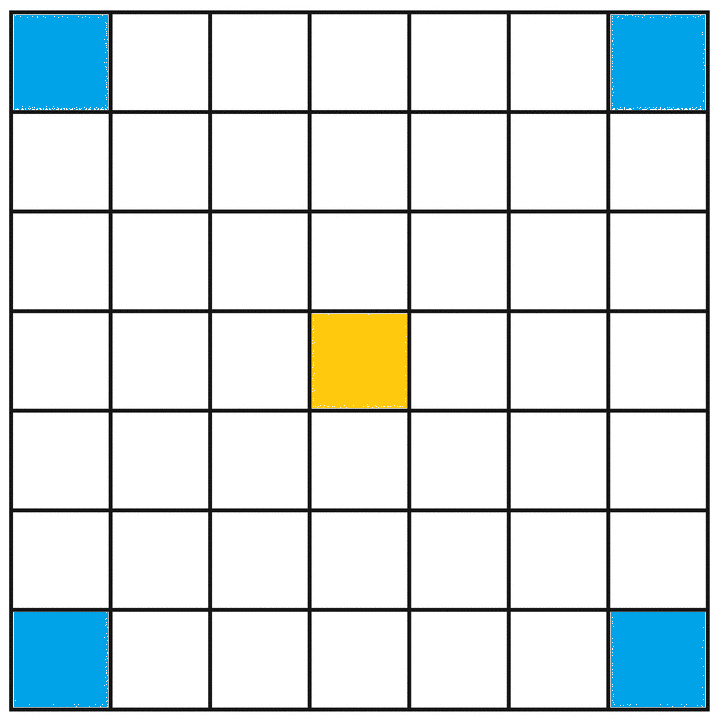
\includegraphics[width=4cm]{figures/structure/7_grid_center_corner.png}
        \caption{Center and corner cubes}\label{fig:7-center-corner}
    \end{minipage}
    \begin{minipage}{0.45\textwidth}
        \centering
        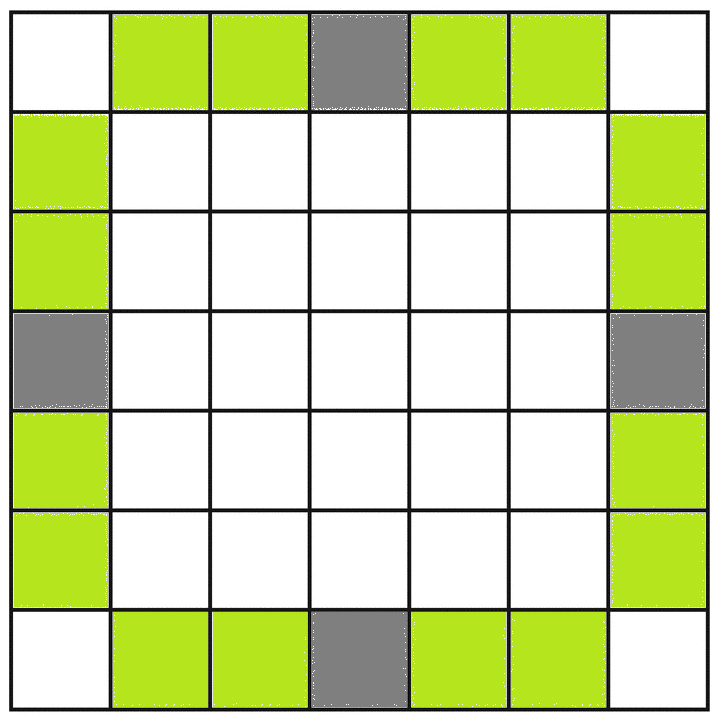
\includegraphics[width=4cm]{figures/structure/7_grid_edge.png}
        \caption{Edge cubes}\label{fig:7-edge}
    \end{minipage}
\end{figure}
In Figure~\ref{fig:7-edge}, we are showing the two types of edge cubes. The ones colored in green are called \textit{wing edges} and the ones colored in grey are called \textit{middle edges}. Clearly, when we shuffle the cube, the middle edge will only permute with other middle edges and the wing edges will permute with other wing edges. The middles edges in $C_7$ generate exactly the same amount of permutations and orientations as they are in $C_3$. We can further split the wing edges into two sets as shown in Figure~\ref{fig:7-wing-edge}. The yellow wing edges will only permute with other yellow wing edges and the blue ones will permute with other blue ones. For an arbitrary large cube $C_n$, we can calculate the number of sets of wing edges it has by finding $\lfloor \frac{n - 2}{2} \rfloor$ and each set of wing edges has $2 \cdot 12 = 24$ small cubes. Due to the inner structure of Rubik's Cubes, different from the middles edges, each one of the wing edges has only one possible orientation when it is at fixed locations.
\begin{figure}[ht]
    \centering
    \begin{minipage}{0.45\textwidth}
        \centering
        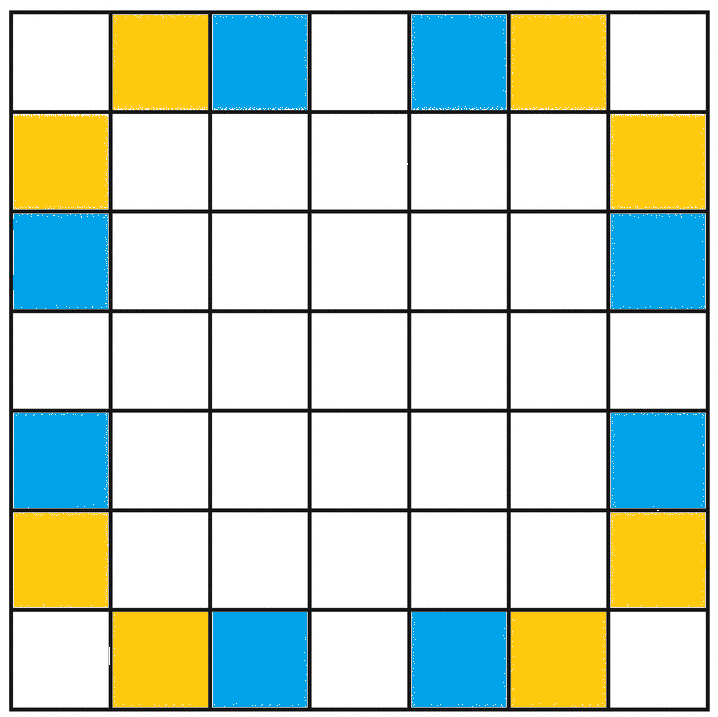
\includegraphics[width=4cm]{figures/structure/7_grid_wing_edge.png}
        \caption{Wing edges}\label{fig:7-wing-edge}
    \end{minipage}
    \begin{minipage}{0.45\textwidth}
        \centering
        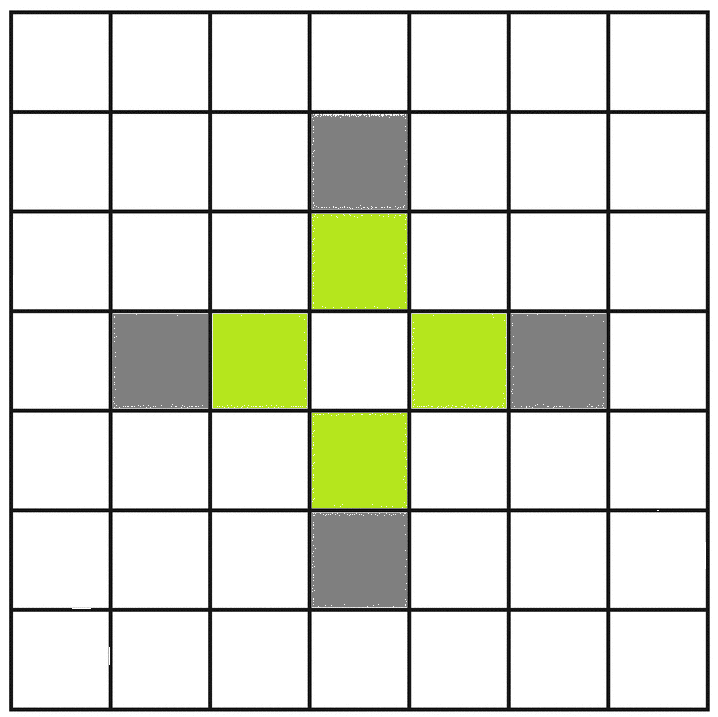
\includegraphics[width=4cm]{figures/structure/7_grid_plus_center.png}
        \caption{$+$ centers}\label{fig:7-plus-center}
    \end{minipage}
\end{figure}
\par Besides the fixed centers, there are three more types of small cubes with only one visible piece we want to introduce. The ones displayed in Figure~\ref{fig:7-plus-center} are called the ``\textit{$+$ centers}'' since they form the $+$ shape. Similar to the wing edges, they can be further split into two sets and those pieces only permute with same colored ones. Secondly, we want to show the ``\textit{$\times$ centers}''. As displayed in Figure~\ref{fig:7-x-center}, those pieces form the $\times$ shape and they can be split to two sets as well.
\begin{figure}[ht]
    \centering
    \begin{minipage}{0.45\textwidth}
        \centering
        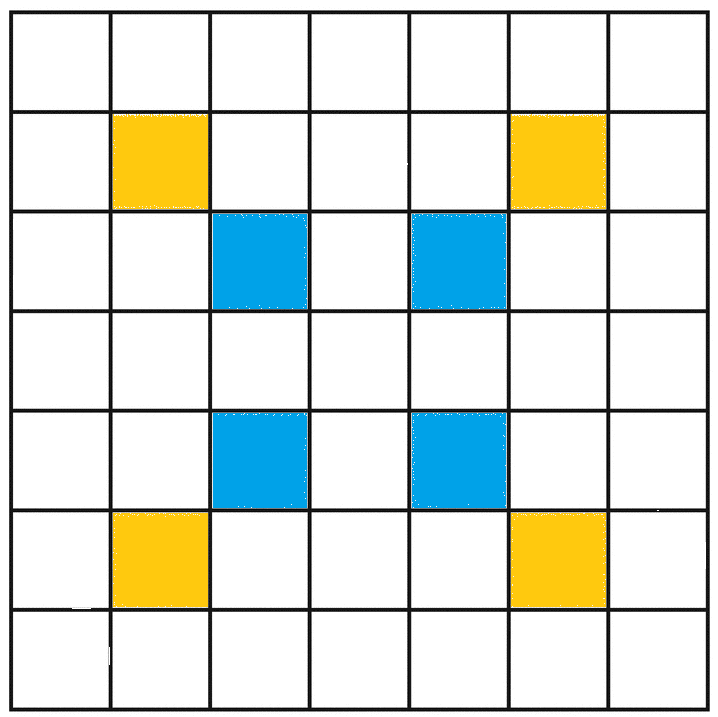
\includegraphics[width=4cm]{figures/structure/7_grid_x_center.png}
        \caption{$\times$ centers}\label{fig:7-x-center}
    \end{minipage}
    \begin{minipage}{0.45\textwidth}
        \centering
        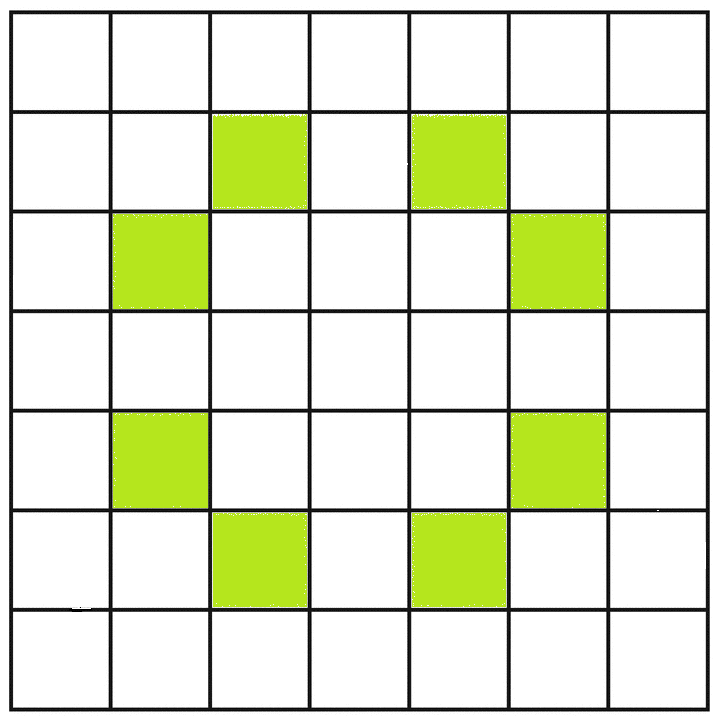
\includegraphics[width=4cm]{figures/structure/7_grid_oblique_center.png}
        \caption{Oblique centers}\label{fig:7-oblique-center}
    \end{minipage}
\end{figure}
The number of sets of $+$ centers and $\times$ centers of an arbitrarily large cube $C_n$ can be calculated by the equation defined above for wing edges, and each set of $+$ centers or $\times$ centers contains $4 \cdot 6 = 24$ small cubes. Finally, the pieces that are not covered by the $+$ shape and the $\times$ shape are denoted the oblique centers. They are displayed in Figure~\ref{fig:7-oblique-center}. Though these three type of centers pieces are different, they permute in a similar fashion; they can change their locations freely but not their orientations.
\par We can further differentiate odd cubes and even cubes. Since $C_7$ is an odd cube, all types of small cubes exist within it. For an even cube, there will be no middle edges and ``$+$ centers'' since the fixed center piece does not exist. Therefore, there is no preferred orientation of an even cube, and some sequences of fundamental movements will be equivalent to rotating the entire cube in a three-dimensional space. Thus, the number of permutations is reduced by a factor of 24. This is because all 24 possible positions and orientations of the first corner are equivalent because of the lack of fixed centres. After addressing all types of small cubes and the difference between odd and even cubes, we now have all the tools we need to calculate group size of $G_n$ for an arbitrary cube $C_n$. In Table~\ref{tab:permutation}, we show details of this calculation. 
\begin{table}[ht]
    \centering
    \begin{tabular}{|p{3cm}|p{11cm}|}
        \hline Type of cube & Number of orderings \\ \hline
        \hline Corner cubes & All cubes can arrange their corners in $8! \cdot 3^7$ different ways.  \\ 
        \hline Middle edges & All odd cubes can arrange their middles edges in $12! \cdot 2^{10}$ ways. Since even cube does not have middle edges, an arbitrary cube $C_n$ has $(12! \cdot 2^{10})^{n \mod 2}$ ways to order its middles edges. \\ 
        \hline Wing edges & An arbitrary cube $C_n$ has $(24!)^{\lfloor \frac{n - 2}{2} \rfloor}$ ways to order its wing edges. \\ 
        \hline Fixed centers & Only odd cubes have fixed centers and since they are fixed, they do not any anymore possible orderings to the calculation. \\ 
        \hline \pbox{3cm}{\vspace*{0.1cm} ``$+$ centers'' \\ ``$\times$ centers'' \\  Oblique centers \vspace*{0.1cm}} & \vspace*{-0.8cm} Since those center pieces permute in a similar fashion, we can put them together to calculate the number of orderings they generate. The details of this calculation can be found in paper\cite{size} and the result is given as $(\frac{24!}{(4!)^6})^{\lfloor (\frac{n - 2}{2})^2 \rfloor}$. \\ \hline
    \end{tabular}
    \caption{Number of permutation different type of small cubes generates}\label{tab:permutation}
\end{table}
Finally we can put everything together and the order of group $G_n$ for states of an arbitrary Rubik's Cube $C_n$ can be calculated by the following function:
$$f(n) = 8! \cdot 3^7 \cdot (12! \cdot 2^{10})^{n \mod 2} \cdot (24!)^{\lfloor \frac{n - 2}{2} \rfloor} \cdot (\frac{24!}{(4!)^6})^{\lfloor (\frac{n - 2}{2})^2 \rfloor} \cdot 24^{-((n + 1) \mod 2)}$$
In Table~\ref{tab:cube-size}, we show some calculations we obtained by using the equation above to demonstrate how fast the corresponding group size increases when the side length of a Rubik's Cube increase.
\begin{table}[ht]
    \centering
    \begin{tabular}{|c|c|}
        \hline Cube group & Group size \\
        \hline $G_3$ & $4.325 \times 10^{19}$ \\
        \hline $G_4$ & $7.401 \times 10^{45}$ \\
        \hline $G_5$ & $2.829 \times 10^{74}$ \\
        \hline $G_6$ & $1.572 \times 10^{116}$ \\
        \hline $G_7$ & $1.950 \times 10^{160}$ \\ \hline
    \end{tabular}
    \caption{Group size of different Rubik's Cubes}
    \label{tab:cube-size}
\end{table}
This quantifies our claim in Chapter~\ref{chap:encryption} that the key space explodes as the size of our cube increases. The function $f(n)$ gives us the size of an arbitrary $G_n$, but the exact algebraic structure is not known for $n > 3$.

\section{Semi-direct product of a group}
The group structure of $G_3$ is well understood and it can be expressed as a semi-direct product of other common groups such as the cyclic group. Before we show how to represent $C_3$, we need to review some group theory knowledge, and some definitions here will help in understanding the key exchange protocol in Chapter~\ref{chap:exchange} as well. 
\begin{definition} A function $\phi$ from a group $G$ to a group $H$ is a \textbf{homomorphism} if $\phi$ preserves the group operation; that is if $\phi(ab) = \phi(a)\phi(b)$ for all $a, b \in G$.
\end{definition}
\begin{definition} An \textbf{isomorphism} is a homomorphism $\phi$ from a group $G$ to a group $H$ that is one-to-one and onto.
\end{definition}
\begin{definition} An \textbf{automorphism} is an isomorphism from a group $G$ onto itself. The set of automorphisms of a group $G$ is denoted by $Aut(G)$.
\end{definition}
\begin{definition} The \textbf{alternating group}, denoted $A_n$ is the group of all even permutations in $S_n$.
\end{definition}
\begin{definition} Let $G$ be a group and $H$ be a subgroup of $G$, the subgroup $H$ is a \textbf{normal subgroup} of $G$, denoted by $H \triangleleft G$, if $\forall g \in G$, $gH = Hg$.
\end{definition}
\begin{definition} Let $G$ and $H$ be two groups. Then the \textbf{direct product} of $G$ and $H$ is the group $G \times H$ under the operation $(g_1, h_1) \cdot (g_2, h_2) = (g_1g_2, h_1h_2)$ where $g_1,g_2 \in G$ and $h_1,h_2 \in H$.
\end{definition}
\begin{definition} Let $H_1$ and $H_2$ be two subgroups of $G$, then $G = H_1 \rtimes H_2$ is a \textbf{semi-direct product} if:
    \begin{enumerate}
        \item $G = H_1H_2$.
        \item $H_1 \cap H_2 = e$, where $e$ is the identity element of $G$.
        \item $H_1 \triangleleft G$.
    \end{enumerate}
\end{definition}
\par We can now describe the group structure of $G_3$. A complete proof can be found in \cite{janet}, but we will sketch the details here. Let us consider two subgroups of $G_3$. First the subgroup $H_1$ of cube orientations, which leave the position of every small cube fixed but can change their orientations. One can show this subgroup is a normal subgroup of $G$. It can be represented by moves that flip a few edges or twist corners. For example, the move ``$R\,U\,D\,B2\,U2\,B'\,U\,B\,U\,B2\,D'\,R'\,U'$ '' flips two edges. The structure of this group is $\mathbb{Z}_3^7 \times \mathbb{Z}_2^{11}$ since the group of rotations of each corner is a cyclic group of order $3$ and we mentioned that we can determine orientations of 7 among 8 corner cubes freely and the last one will be fixed. The argument for flipping edges is exactly the same.
\par In addition, we take the subgroup $H_2$ which permutes the positions of the small cubes but does not change their orientations. Similar to above, this group can be represented by a direct product of two subgroups, which are the group of permutations on the corners $S_8$ and the group of even permutations on the edges $A_{12}$ (because of the even parity). Hence the structure of $H_2$ is $S_8 \times A_{12}$. Notice that here we do not mind if $H_2$ is a normal subgroup or not.
\par Clearly $H_1 \cap H_2 = e$, where $e$ is the identity in $G_3$, since $H_1$ keeps all small cubes fixed but changes their orientations, whereas $H_2$ always moves the cubes. Since $H_1$ and $H_2$ account for all possible change on the cube $C_3$, $H_1H_2$ can form the entire group $G_3$. It follows that the cube group $G_3$ is isomorphic to the semi-direct product of these two groups:
$$G_3 = H_1 \rtimes H_2 \cong (\mathbb{Z}_3^7 \times \mathbb{Z}_2^{11}) \rtimes (S_8 \times A_{12})$$
By finding the group order of above semi-direct product, we will again retrieve the same result we found earlier in this chapter. For instance, the largest order of an element in $G_3$ is 1260 and one such element is ``$R\,U2\,D'\,B\,D'$ ''\cite{order}. However, we have not yet found a efficient method to generalize those results to other Rubik's Cube groups $G_n$.
\par In this chapter, we introduced methods to find group size of $G_n$ of an arbitrary large cube $C_n$. The explosion of the group sizes we observed suggests that larger cubes may make brute force attacks more computationally expensive. Although not known for larger cubes, we are able to give the isomorphism class for $G_3$. Since this additional structure is known, it could open up the door to opportunities to further reduce computation cost of the brute attacks on encryption based on $C_3$.